\documentclass{article}
\usepackage[left=25mm,right=25mm,bottom=35mm]{geometry}
\usepackage{amsmath,graphicx}
\usepackage[comma,numbers,square,sort&compress]{natbib}

\begin{document}

\title{Fault Diagnosis of Pitch Sensor Bias for Wind Turbine Based on the Multi-Innovation Kalman Filter}

\author{Dinghui WU,
        Yiyang LI,
        Zhicheng JI}
\date{}
\maketitle


\begin{abstract}
This paper presents a fault diagnosis method for detecting pitch sensor
offset fault according to the mechanical structure characteristics of wind turbine.
The method establishes corresponding relation between the change of pitch angle
and the minute displacement which produced by the force acting on tower of
wind turbine. It is based on the change of displacement to diagnosis whether
the fault occurs. With regard to the large noise of sensors, we adopt the
multi-innovation Kalman filter to enhance the estimation accuracy and
convergence speed. The simulation results show that the multi-innovation
Kalman filter based method can diagnose the fault effectively and is
better than the common Kalman filter.
\end{abstract}

\footnotetext{\\
Key laboratory of Advanced Process Control for Light Industry, Ministry of Education, Jiangnan University, Wuxi, 214122, China\\
Corresponding author:\\
Dinghui Wu, Key laboratory of Advanced Process Control for Light Industry, Ministry of Education, Jiangnan University, Wuxi 214122, China\\
Email: wh033098@163.com\\
This research was supported by Prospective Joint Research Project of Industry, Education and Academy of Jiangsu Province (BY2012071) and China Postdoctoral Science Foundation (2013M531272).}




\section{Introduction}


Wind energy is playing a more and more important role in world power
production \cite{ref:1}. Since most wind farms are located in desert or sea
areas where the natural environment is harsh \cite{ref:2},
wind turbines often have faults. Modern wind turbines often adopt fault
tolerant control methods to maintain normal operation, and fault
diagnosis is the premise and necessary condition \cite{ref:3}. The variable pitch
system is an important part of wind turbines, the pitch fault
will affect the generated power when the wind velocity is above the rated
one, when the wind velocity is below the rated one, the pitch fault has
a little impact on the generated power.

There have been many fault diagnosis methods for wind turbines.
Watson et al. has studied the rotor fault based on the wavelet analysis,
the analysis involves monitoring the power output and processing the data to
obtain the magnitude of particular frequency components \cite{ref:4}. This method
can extract the characteristic of fault, however, the wavelet analysis
must be calculated off-line, which limits the widespread applications.
Guo et al. has studied the current feedback sensor fault, speed sensor
fault and constant gain output fault of wind turbine control system\cite{ref:5}.
The neural networks are trained to analyze fault conditions by selecting
the appropriate eigenvalue and training samples. But the neural networks
algorithm relies on a large number of training samples, which is not
available in remote areas. Some faults do not
change system structures, but will affect the system parameters, we can
set up the linear model of the turbines, and the fault information can be
reflected on the parameters' change. So, the system identification
technology can be adopted to fault detection and diagnosis \cite{ref:6}.




When the wind velocity is above the rated one, the control objective
is to maintain constant generated power \cite{ref:7}, the objective is realized by
adjusting the angle of three pitches. The pitch angle sensor is an
important part of the closed-loop pitch system, if an offset fault
happens to pitch angle sensors, the whole pitch system will become
unstable. Under the effective wind velocity, there will be a thrust
acting on the rotor, the thrust makes the tower sway back and forth \cite{ref:8},
which results in a tiny displacement. The value of thrust dependents
on the thrust coefficient, and the thrust coefficient relies on the pitch
angle and tip-speed ratio, therefore, the pitch angle will influence
the thrust. A corresponding relationship can be formed between the
pitch angle and the tiny displacement, but the pitch sensor fault
will break the relationship. As a consequence, the fault can be
detected by monitoring the relationship.

The above method involves a lot of data processing, the
Kalman filter based on the multi-innovation method is utilized to filter the
value obtained from the pitch angle sensor and tower displacement
sensor. The multi-innovation algorithm extends the scalar value \cite{ref:9,ref:10,ref:11},
and uses not only the current data but
the past data as well, which significantly improves the accuracy of the
estimate and the convergence speed \cite{ref:12}. The tower displacement
calculated from pitch angle and the displacement from sensor should
 be equal when the pitch angle sensor is normal. When there is a
 deviation between two displacements, we can detect a fault.

The rest of this paper is organized as follows. Section 2 gives the wind
turbine model for simulation, and presents the fault model for
analysis. Section 3 gives the fault diagnosis and data processing
procedure using the multi-innovation Kalman filter. Section 4
contains a simulation result. Finally, concluding remarks are given in Section 5.

\section{Wind Turbine Model}


\subsection{Aerodynamic Model}

The wind energy captured from the three blades is transformed
to the rotational motion of the rotor, the rotor speed is $\omega_r(t)$.
The captured wind energy is dependent on the effective wind speed
$v_r(t)$, the air density $\rho$ and the rotor swept area $A$ and
the power coefficient $C_p(\lambda(t),\beta(t))$. The power
coefficient relies on tip-speed ratio $\lambda(t)$ and pitch
angle $\beta(t)$. The aerodynamic torque $T_a(t)$ applied to
the rotor by blade can be obtained from tip-speed ratio $\lambda(t)$
and blade radius $r$ \cite{ref:13}, as illustrated below
\begin{eqnarray}
  \lambda(t) &=& \frac{r\omega_r(t)}{v_r(t)}, \\
  T_a(t) &=& \frac{1}{2\omega_r(t)} \rho A v_r^3 C_p(\lambda(t),\beta(t)).
\end{eqnarray}



\subsection{Tower Model}

The wind acting on each blade results in a
thrust on the rotor, which can be calculated as \cite{ref:14}
\begin{equation} \label{eq.aero}
  F_t(t) = \frac{1}{2} \rho A v_r^2(t)C_t(\lambda(t),\beta(t)).
\end{equation}

The thrust coefficient  $C_t(\lambda(t),\beta(t))$ is
dependent on  $\lambda(t)$ and $\beta(t)$ .

The resulting tower force  $F_{th}(t)$ on the tower at hub
height $h$ depends on the azimuth angle of rotor, which
is the synthesis of three thrusts \cite{ref:8}
\begin{eqnarray}
  F_{th}(t) &=& \sum^{3}_{i=1}F_{th,i}(t) \label{eq.towerforce}, \\
  F_{th,i}(t) &=& F_{t,i}(t)(1+\frac{r_t}{h}\mathrm{cos}(\Psi_i(t))) \label{eq.thrust},
\end{eqnarray}
where $F_{t,i}$ is the thrust from blade $i$, $r_i$ is the
 distance from the hub to the point where the thrust acts on the blade.
 The relationship between $\Psi_1(t)$ , $\Psi_2(t)$ , $\Psi_3(t)$
  and the location of the blades are illustrated in Fig. \ref{fig:position}.
From (\ref{eq.towerforce}) and (\ref{eq.thrust}), it is shown that the location of the blades affects the tower
  force components, which is  different from the aerodynamic torque.

\begin{figure}[!htb]
  \centering
  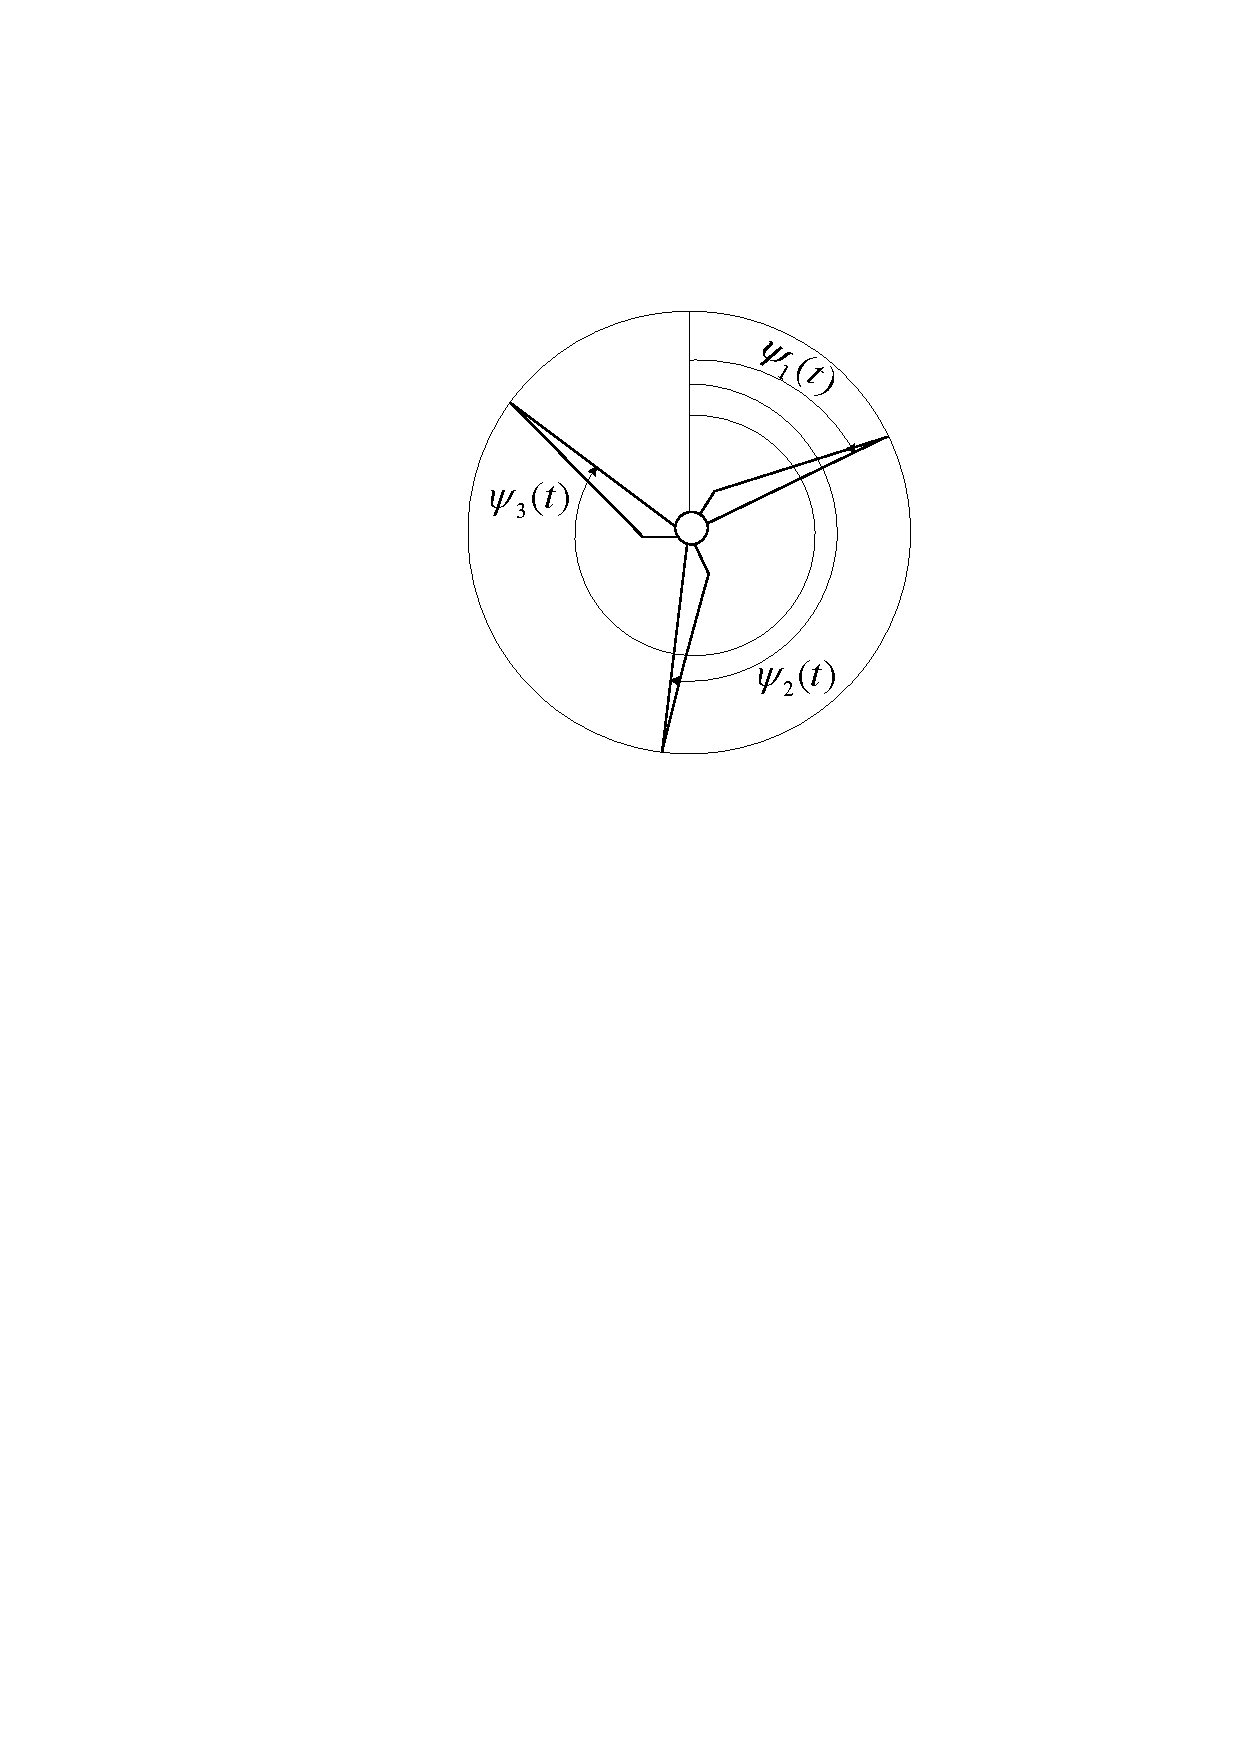
\includegraphics[width=0.4\hsize]{Visio-bladelocation.pdf}
  \caption{Position of blades}
  \label{fig:position}
\end{figure}

Under the tower force, the tower will produce a tiny
displacement  $x_t(t)$. Due to the fact that $x_t(t)$ is the only measured variable in the tower
 model, the movement of the tower can be described as a linear
 displacement of the nacelle. An illustration of this model is given in Fig. \ref{fig:damping},
using a spring-damper terminology the tower model is
 given as
\begin{equation} \label{eq.tower}
  M_t\ddot{x}_t(t) = F_{th}(t) - B_t\dot{x}_t(t) - K_tx_t(t),
\end{equation}
where $M_t$ is the top mass of the tower, $B_t$  is the
tower damping coefficient, $K_t$  is the tower torsion coefficient.

\begin{figure}[!thb]
  \centering
  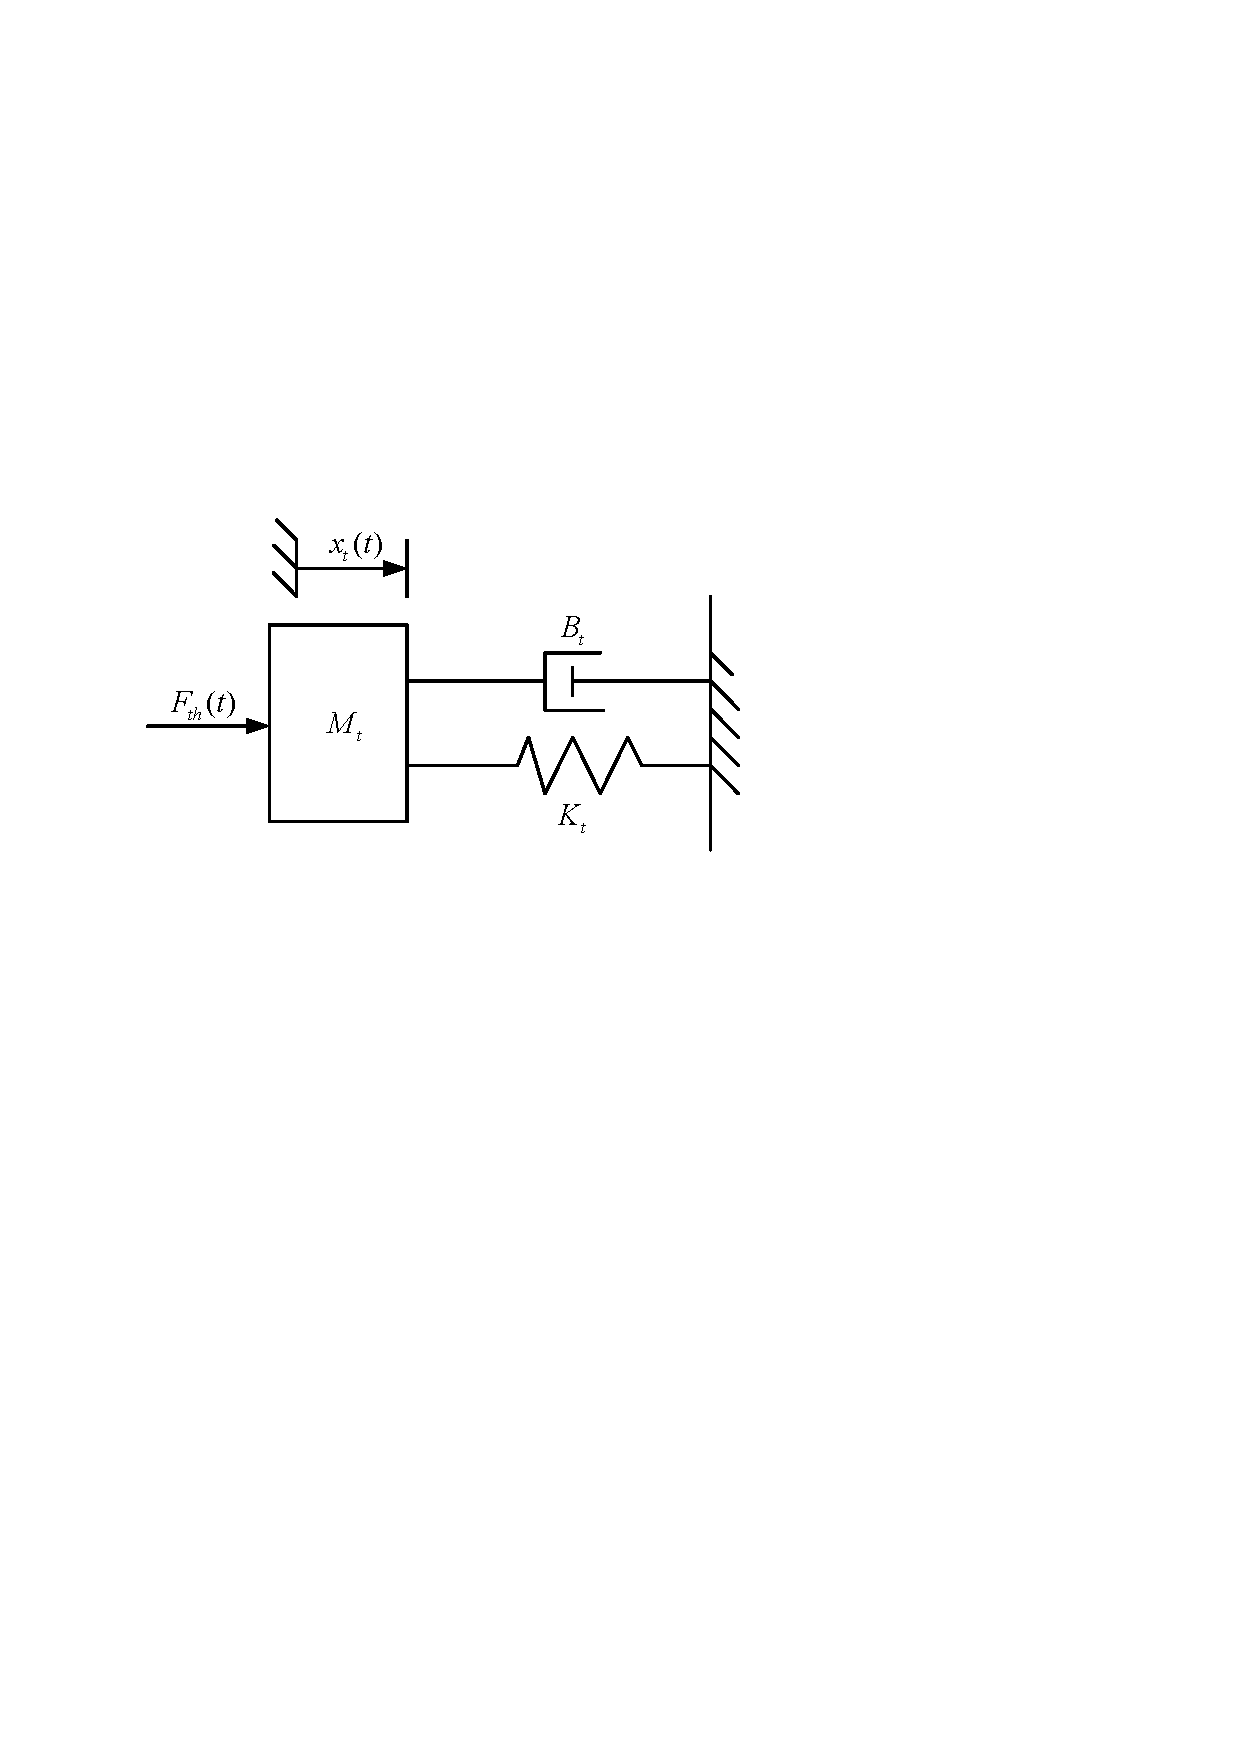
\includegraphics[width=0.55\hsize]{Visio-damping.pdf}
  \caption{Tower model}
  \label{fig:damping}
\end{figure}

\subsection{Pitch Model}

The pitch actuator is modeled as a second order system \cite{ref:15},
\begin{eqnarray}
  \frac{\beta(s)}{\beta_{ref}(s)} &=& \frac{\omega_n^2}{s^2+2\varsigma\omega_n{}s + \omega_n^2}, \\
  \ddot{\beta}(t) &=& 2\varsigma\omega_n\dot{\beta}(t) - \omega_n^2\beta(t) + \omega_n^2\beta_{ref}(t), \\
  \beta_m(t) &=& \beta(t) + v_\beta(t),
\end{eqnarray}
where $\beta_{ref}(t)$  is the reference to the pitch angle,
$\omega_n$ is the natural frequency of the pitch actuator model,
$\varsigma$ is the damping ratio of the pitch actuator model,
$\beta_m(t)$ is the value returned from the pitch angle sensor
and  $v_\beta$ is the measurement noise.

When an offset pitch angle fault happens, the model of the
actuator is
\begin{eqnarray}
  \ddot{\beta}(t) &=& -2\varsigma\omega_n\dot{\beta}(t) - \omega_n^2(\beta(t)+\beta_{bias}(t))+\omega^2_n\beta_{ref}(t), \\
  \beta_m(t) &=& \beta(t) + \beta_{bias}(t) + v_\beta(t).
\end{eqnarray}
where $\beta_{bias}(t)$ is the offset added to the pitch angle sensor output.

\section{Fault Diagnosis Algorithm }
\subsection{Structure of the Diagnosis System}

A fault diagnosis structure is designed for the pitch system,
which is illustrated in Fig.\ref{fig:faultstructure}.

\begin{figure}[!htb]
  \centering
  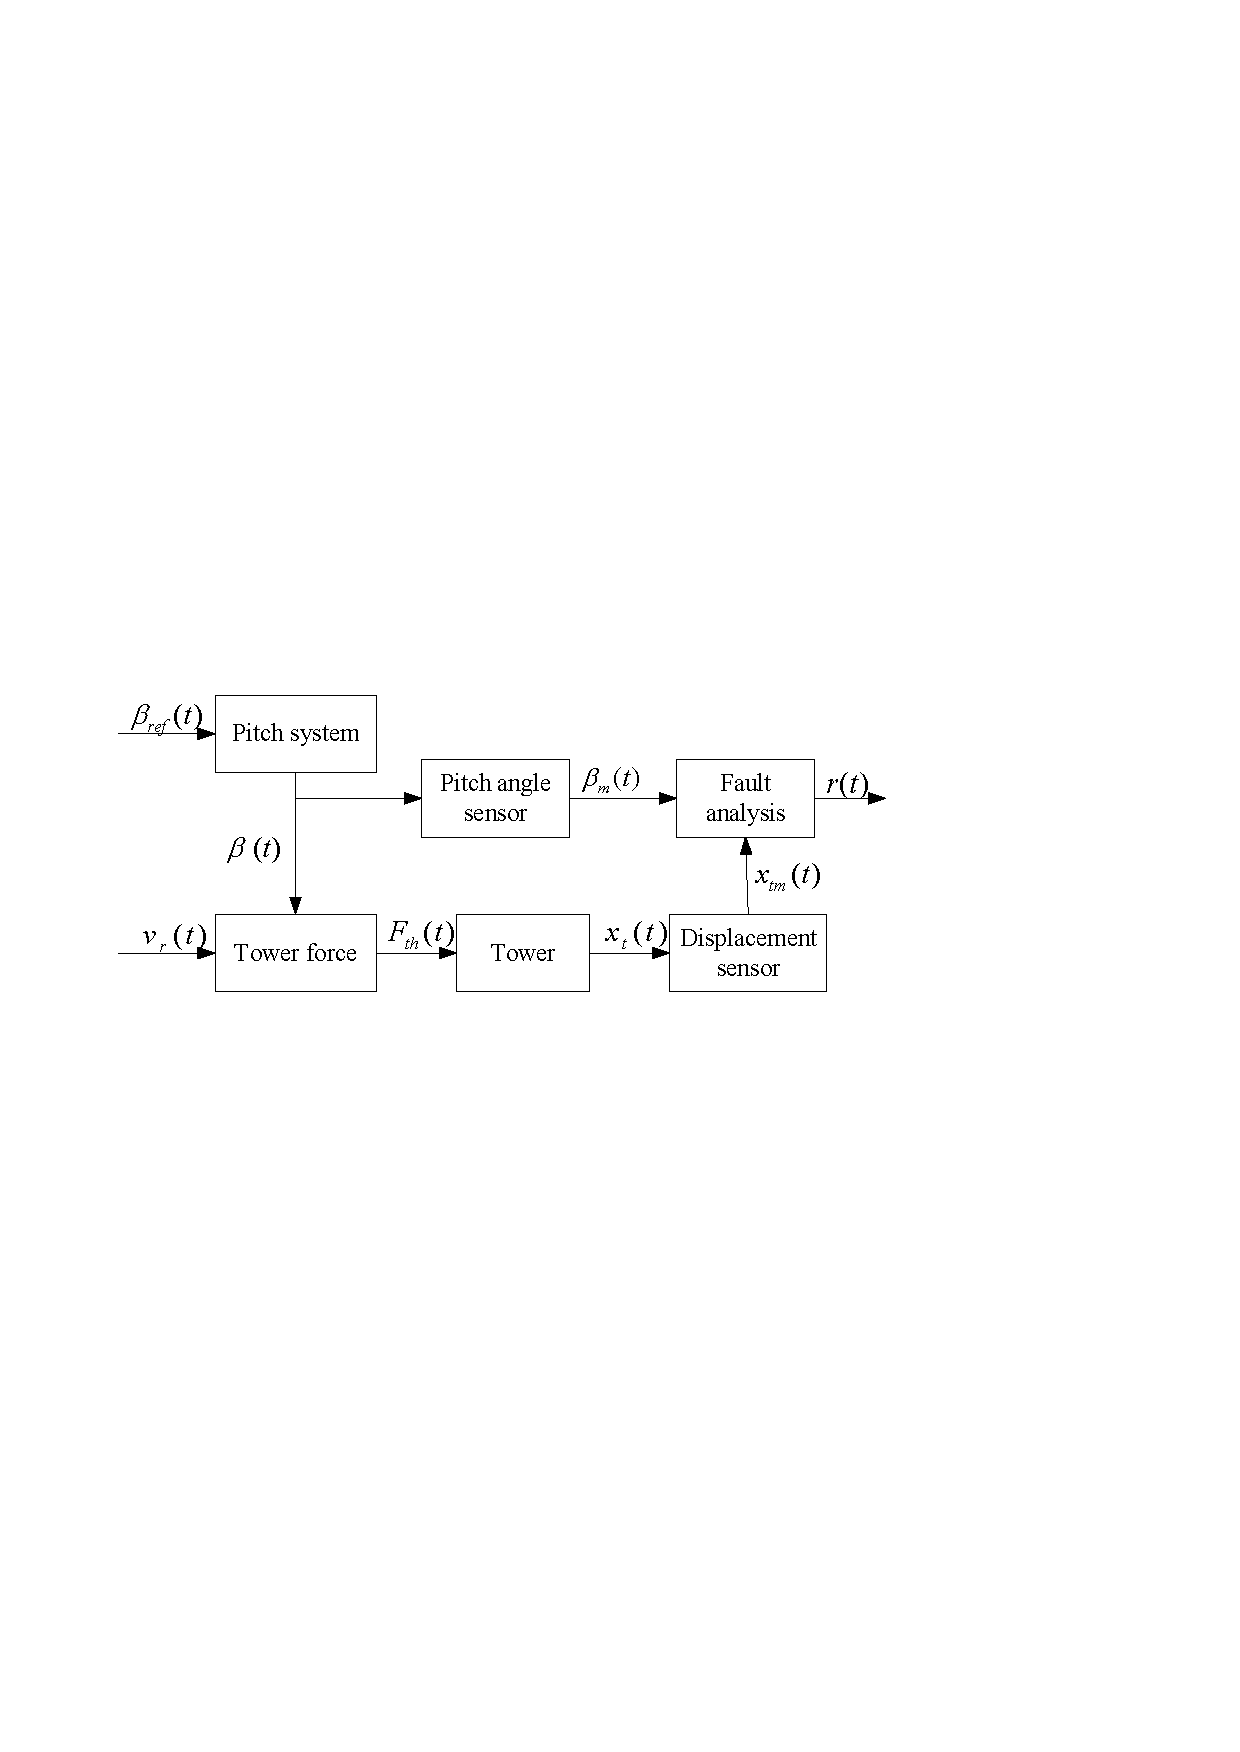
\includegraphics[width=0.8\hsize]{Visio-faultstructure.pdf}
  \caption{Structure of the diagnosis system}
  \label{fig:faultstructure}
\end{figure}

From (\ref{eq.aero}), the thrust $F_t(t)$ on
blade   is related to the thrust coefficient $C_t$ , and the coefficient $C_t$
is related to  $\lambda(t)$ and $\beta(t)$. The tower force $F_{th}(t)$
can be deduced from (\ref{eq.towerforce}) and (\ref{eq.thrust}).
Using (\ref{eq.tower}), we can obtain the tiny displacement $x_t(t)$
 from the tower force $F_{th}(t)$ . An offset in pitch angle will result
 in a small change in thrust coefficient, and the tower force will change
 correspondingly.
As a result, by monitoring the variation of displacement, the fault can be detected.


To maintain a constant wind power output, the closed-loop pitch system works
continuously to obtain the pitch angle objective $\beta_0$. If there
is a constant offset output $-\theta$  adding to the pitch angle sensor,
the sensor output will become $\beta_m = \beta_0 - \theta$ . For the pitch control system,
the value from measurement does not match the control objective, so under
the action of the pitch actuator, the pitch is adjusted  to force the sensor output
back to the objective, that is $\beta'_m=\beta_m + \theta = \beta_0$ . Due to the
offset in the sensor output, the real pitch angle is  $\beta=\beta'_m+\theta=\beta_0+\theta$.
Therefore, we draw the conclusion that the measured displacement $x_{tm}$  is
different from the calculated displacement obtained from $\beta_0$. The fault
severity can be concluded by comparing the measured and calculated displacement.

As the wind turbines work in a harsh condition, the value returned from
the sensor is polluted by noise and the displacement caused by
the sensor offset fault is rather small, it is possible for the displacement
 information to be submerged by the noise. It is necessary to filter the
 sensor output, the Kalman filter based on the multi-innovation technology
 is an efficient way to obtain the optimal state estimation, and to realize
the accurate judgement of the sensor offset fault.



\subsection{Kalman Filter Based on Multi-Innovation}

The Kalman filter is a recursive method which estimate the optimal
system states \cite{ref:16}. The Kalman filter consists of two steps: a prediction
step and an update step. In the prediction step, the estimate of the
state at the current time is produced from the previous time.
The predicted step combines the priori prediction with the current
observation information to refine the state estimate.

The innovation is defined as the useful information which can improve parameters
or states estimation accuracy \cite{ref:17}. For the linear discrete system of the
wind turbine,
the conventional Kalman filter can be written as the
following five equations,
\begin{eqnarray}
  \hat{x}_{k|k-1} &=& A_{k-1}\hat{x}_{k-1}, \\
  P_{k|k-1} &=& A_{k-1}P_{k-1}A^T_{k-1} + \Gamma_{k-1}Q_{k-1}\Gamma^T_{k-1}, \\
  \hat{x}_k &=& \hat{x}_{k|k-1} + K_k[z_k - C_k\hat{x}_{k|k-1}], \\
  P_k &=& [I - K_k C_k]P_{k|k-1}, \\
  K_k &=& P_{k|k-1}C^T_k[C_k P_{k|k-1}C^T_k + R_k]^{-1},
\end{eqnarray}
where ${x}_{k|k-1}$ is  posteriori state estimate at time $k$ given
observations up to and including time $k$, $P_{k|k-1}$ is the
posteriori error covariance matrix, $A_{k-1}$ is the state transition matrix
which is applied to the previous state $\hat{x}_{k-1}$, $K_k$ is the
optimal Kalman gain, $\hat{x}_k$ is the updated state estimate, $P_k$ is
the updated estimate covariance matrix, $C_k$ and $Q_k$ is the noise covariance matrix.

The single innovation for the conventional Kalman filter is defined as
\begin{equation}
  c(k) = z_k - C_k\hat{x}_{k|k-1}.
\end{equation}

Then we extend the single innovation to a multi-innovation vector,
\begin{eqnarray}
E(p, k) &=& \begin{bmatrix}
e(k) \\
e(k-1) \\
\vdots \\
e(k-p+1)
\end{bmatrix} \notag\\
&=&
\begin{bmatrix}
z_k - C_k\hat{x}_{k|k-1} \\
z_{k-1} - C_{k-1}\hat{x}_{k-1|k-2} \\
\vdots \\
z_{k-p+1} - C_{k-p+1}\hat{x}_{k-p+1|k-p}
\end{bmatrix},
\end{eqnarray}
where $p$ is the innovation length. Then the updated state estimate is changed to
\begin{eqnarray}
  \hat{x}_k &=& A_{k-1}\hat{x}_{k-1} + [K_{k}, K_{k-1}, K_{k-2}, ... , K_{k-p}] E(p, k) \notag\\
  &=& A_{k-1}\hat{x}_{k-1} + \sum^p_{i=1}K_i(k)e(k-i+1).
\end{eqnarray}

Here we choose $K_i(k) = K(k-i+1)$.

\subsection{Design of the State and Observation Equation}

The measurement of displacement $x_{tm}(k)$ is processed by the multi-innovation
Kalman filter to obtain the optimal state estimate
, which is polluted by noise. Under the random tower force, the wind turbine
is not moving uniformly from the equilibrium position. In order to get the
discretization expression of the displacement and its derivative, the sampling
period $T_0=0.01s$ is taken, it is assumed that within a sampling period of
displacement generated by the wind turbine tower, it moves uniformly.
$x_{tm}(k)$ is the displacement measured at time $kT_0$, by applying the
kinematics formulas, the motion of tower can be obtained as
\begin{eqnarray}
  x_{tm}(k+1) &=& x_{tm}(k) + \dot{x}_{tm}(k)T_0, \\
  \dot{x}_{tm}(k+1) &=& \dot{x}_{tm}(k).
\end{eqnarray}

The displacement and velocity of tower is chosen as the state parameters, then
the system states at time $kT_0$ is
\begin{equation}
  x(k) =
  \begin{bmatrix}
    x_{tm}(k) \\
    \dot{x}_{tm}(k)
  \end{bmatrix}.
\end{equation}

Then the state space model is
\begin{equation}
  \begin{bmatrix}
    x_{tm}(k+1) \\
    \dot{x}_{tm}(k+1)
  \end{bmatrix}
  =
  \begin{bmatrix}
    1 & T_0 \\
    0 & 1
  \end{bmatrix}
  \begin{bmatrix}
    x_{tm}(k) \\
    \dot{x}_{tm}(k)
  \end{bmatrix} + w(k).
\end{equation}

The observation equation is
\begin{equation}
  z(k) =
  \begin{bmatrix}
    1 & 0
  \end{bmatrix}
  \begin{bmatrix}
    x_{tm}(k) \\
    \dot{x}_{tm}(k)
  \end{bmatrix} + v(k).
\end{equation}

The pitch sensor output $\beta_m$ is polluted by noise, the method
utilized to process displacement can be applied here. The pitch
angle changed in a single period is the uniform motion, and the similar
states can be established as
\begin{eqnarray}
  \begin{bmatrix}
    x_{tm}(k+1) \\
    \dot{x}_{tm}(k+1) \\
    \beta_m(k+1) \\
    \dot{\beta}_m(k+1)
  \end{bmatrix}
  &=&
  \begin{bmatrix}
    1 & T_0 & 0 & 0 \\
    0 & 1 & 0 & 0 \\
    0 & 0 & 1 & T_0 \\
    0 & 0 & 0 & 1
  \end{bmatrix}
  \begin{bmatrix}
    x_{tm}(k) \\
    \dot{x}_{tm}(k) \\
    \beta_m(k) \\
    \dot{\beta}_m(k)
  \end{bmatrix} + w(k), \\
  z(k) &=&
  \begin{bmatrix}
    x_{tm}(t) \\
    \beta_m(t)
  \end{bmatrix}
  \begin{bmatrix}
    1 & 0 & 0 & 0 \\
    0 & 0 & 1 & 0
  \end{bmatrix}
  \begin{bmatrix}
    x_{tm}(k) \\
    \dot{x}_{tm}(k) \\
    \beta_m(k) \\
    \dot{\beta}_m(k)
  \end{bmatrix} + v(k).
\end{eqnarray}

The state space model is
\begin{eqnarray}
  x(k+1) = Ax(k) + w(k), \\
  z(k) = C x(k) + v(k),
\end{eqnarray}
where the parameter matrixes are
$  A = \begin{bmatrix}
    1 & T_0 & 0 & 0 \\
    0 & 1 & 0 & 0 \\
    0 & 0 & 1 & T_0 \\
    0 & 0 & 0 & 1
  \end{bmatrix}$,
  $C =   \begin{bmatrix}
    1 & 0 & 0 & 0 \\
    0 & 0 & 1 & 0
  \end{bmatrix}$.

The procedure for the multi-innovation Kalman filter is described as follows:
the optimal state estimate $\hat{x}(k)$ and state covariance matrix $P(k)$  is known
at step $k$, we compute the optimal Kalman gain $K(k)$, innovation $e(k)$,
then choose the appropriate innovation length $p$, the innovation vector is extended
to innovation the matrix $E(p, k)$ and the optimal state estimate $\hat{x}(k+1)$
at step $k+1$ can be calculated.

\section{Simulation}

In this section, the fault diagnosis for the pitch angle sensor offset fault is
simulated. Fig. \ref{fig:observe} is the original observation of the tower displacement,
Fig. \ref{fig:kalman} is the displacement curve of the Kalman filter, and
Fig. \ref{fig:multi}
is the displacement curve of the multi-innovation Kalman filter. It is shown
from the comparison that both the conventional and the multi-innovation Kalman filter
can remove the influence of noise, and the multi-innovation method is more accurate.

The innovation length $p$ introduced by the multi-innovation Kalman filter not
only can improve the estimation accuracy, but also can improve the
convergence speed. But a large innovation length $p$ involves a large amount of
matrix computation. It is illustrated in
Fig. \ref{fig:innolength0} that the innovation length $p=8$ is
an appropriate one.

This algorithm can be used to detect the severity of the fault. The tested
wind velocity is $25\mathrm{m/s}$, in $40\mathrm{s}-100\mathrm{s}$, the fault happens, a offset $-3^\circ$
is added to the pitch angle sensor output. It is shown in
Fig. \ref{fig:fault1} that,  the displacement of tower changes significantly.

In
Fig. \ ref{fig:fault5},
the offset is changed to $-5^\circ$, in $20\mathrm{s}-140\mathrm{s}$,  the wind velocity accelerates
every ten seconds. As the Fig. \ref{fig:fault5} depicted, the tower displacement is related
to the wind velocity.
In Fig. \ref{fig:fault25}, the wind velocity is $25\mathrm{m/s}$, the offset added to
pitch angle output increases every ten seconds. The result shows that the displacement
changes corresponding to the offset.

The relationship between the wind velocity, the pitch angle sensor offset and the tower
displacement is shown in Fig. \ref{fig:3d}.



\begin{figure}[H]
  \centering
  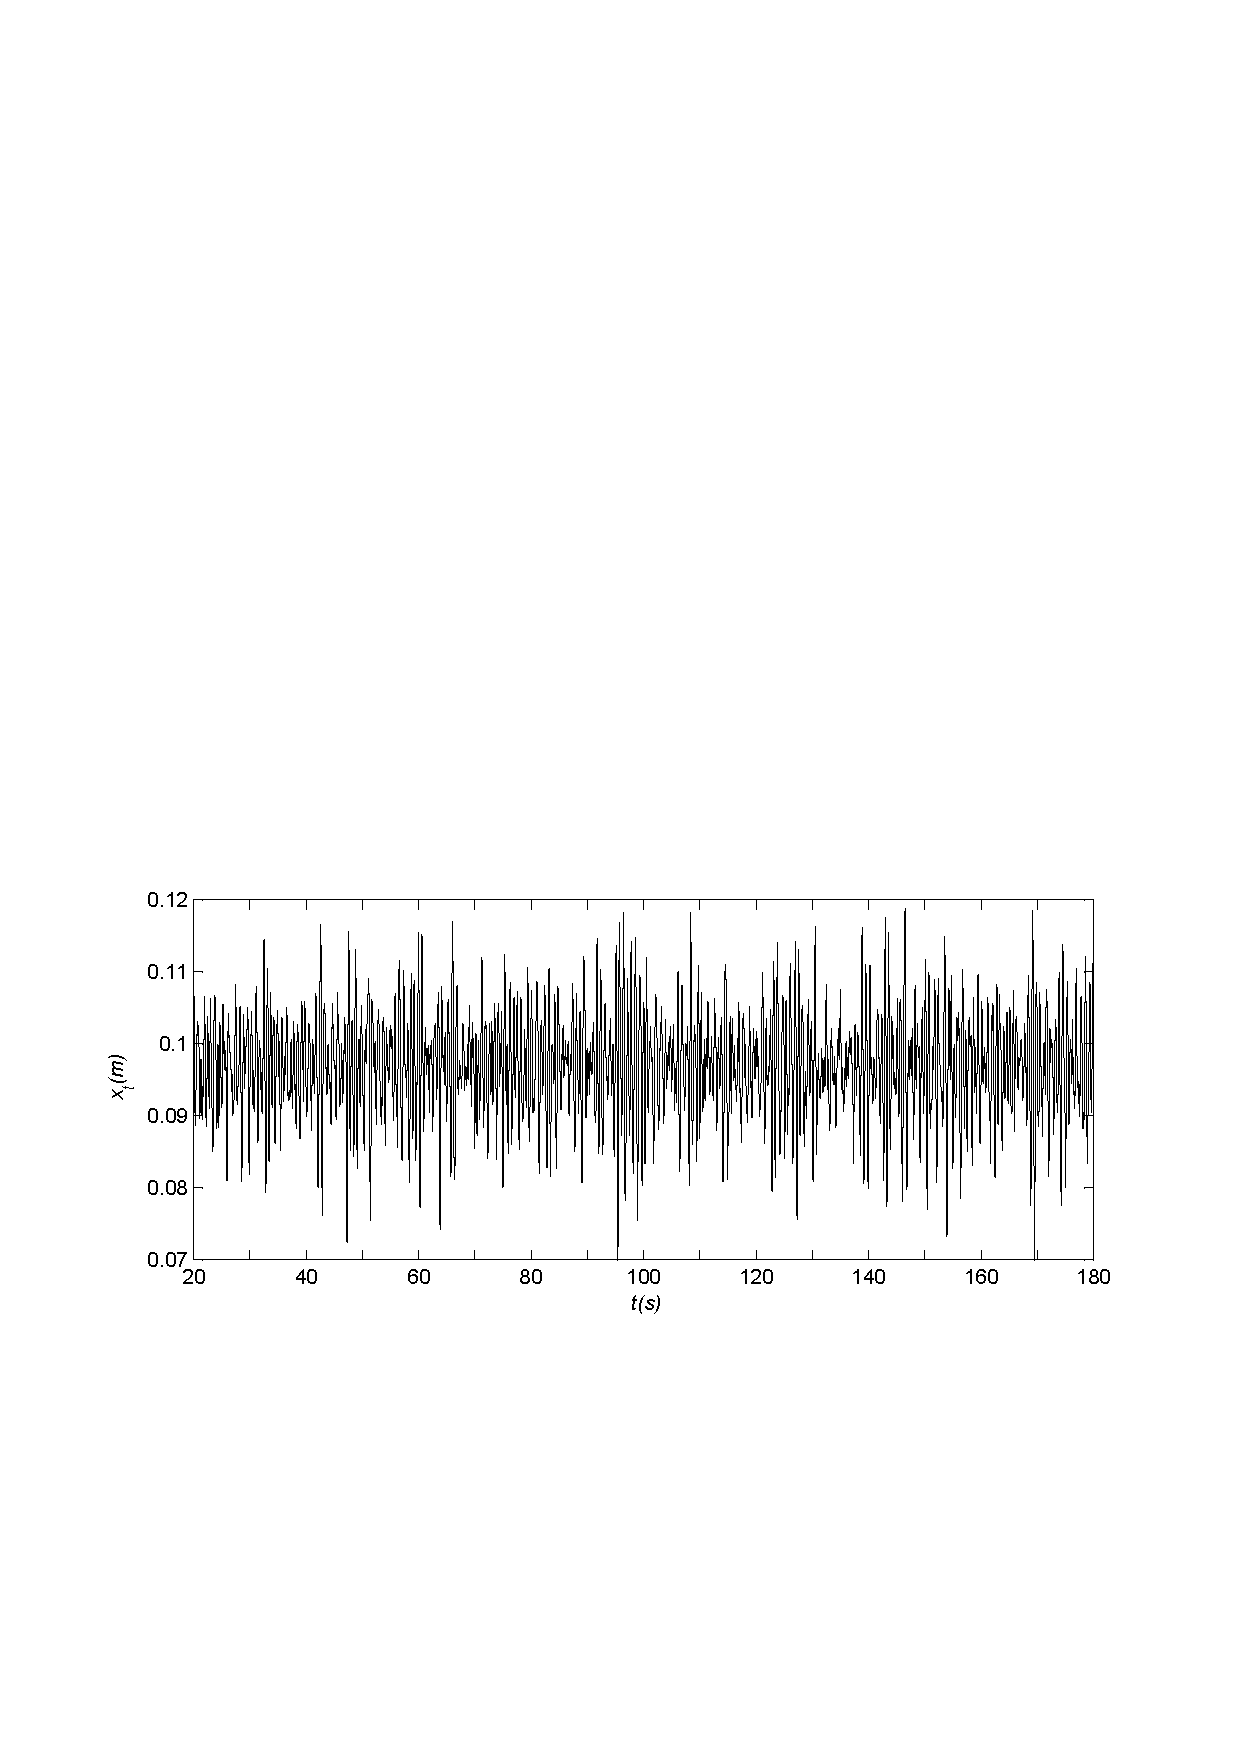
\includegraphics[width=0.8\hsize]{MATLAB-observer.pdf}
  \caption{Observation of displacement}
  \label{fig:observe}
\end{figure}

\begin{figure}[H]
  \centering
  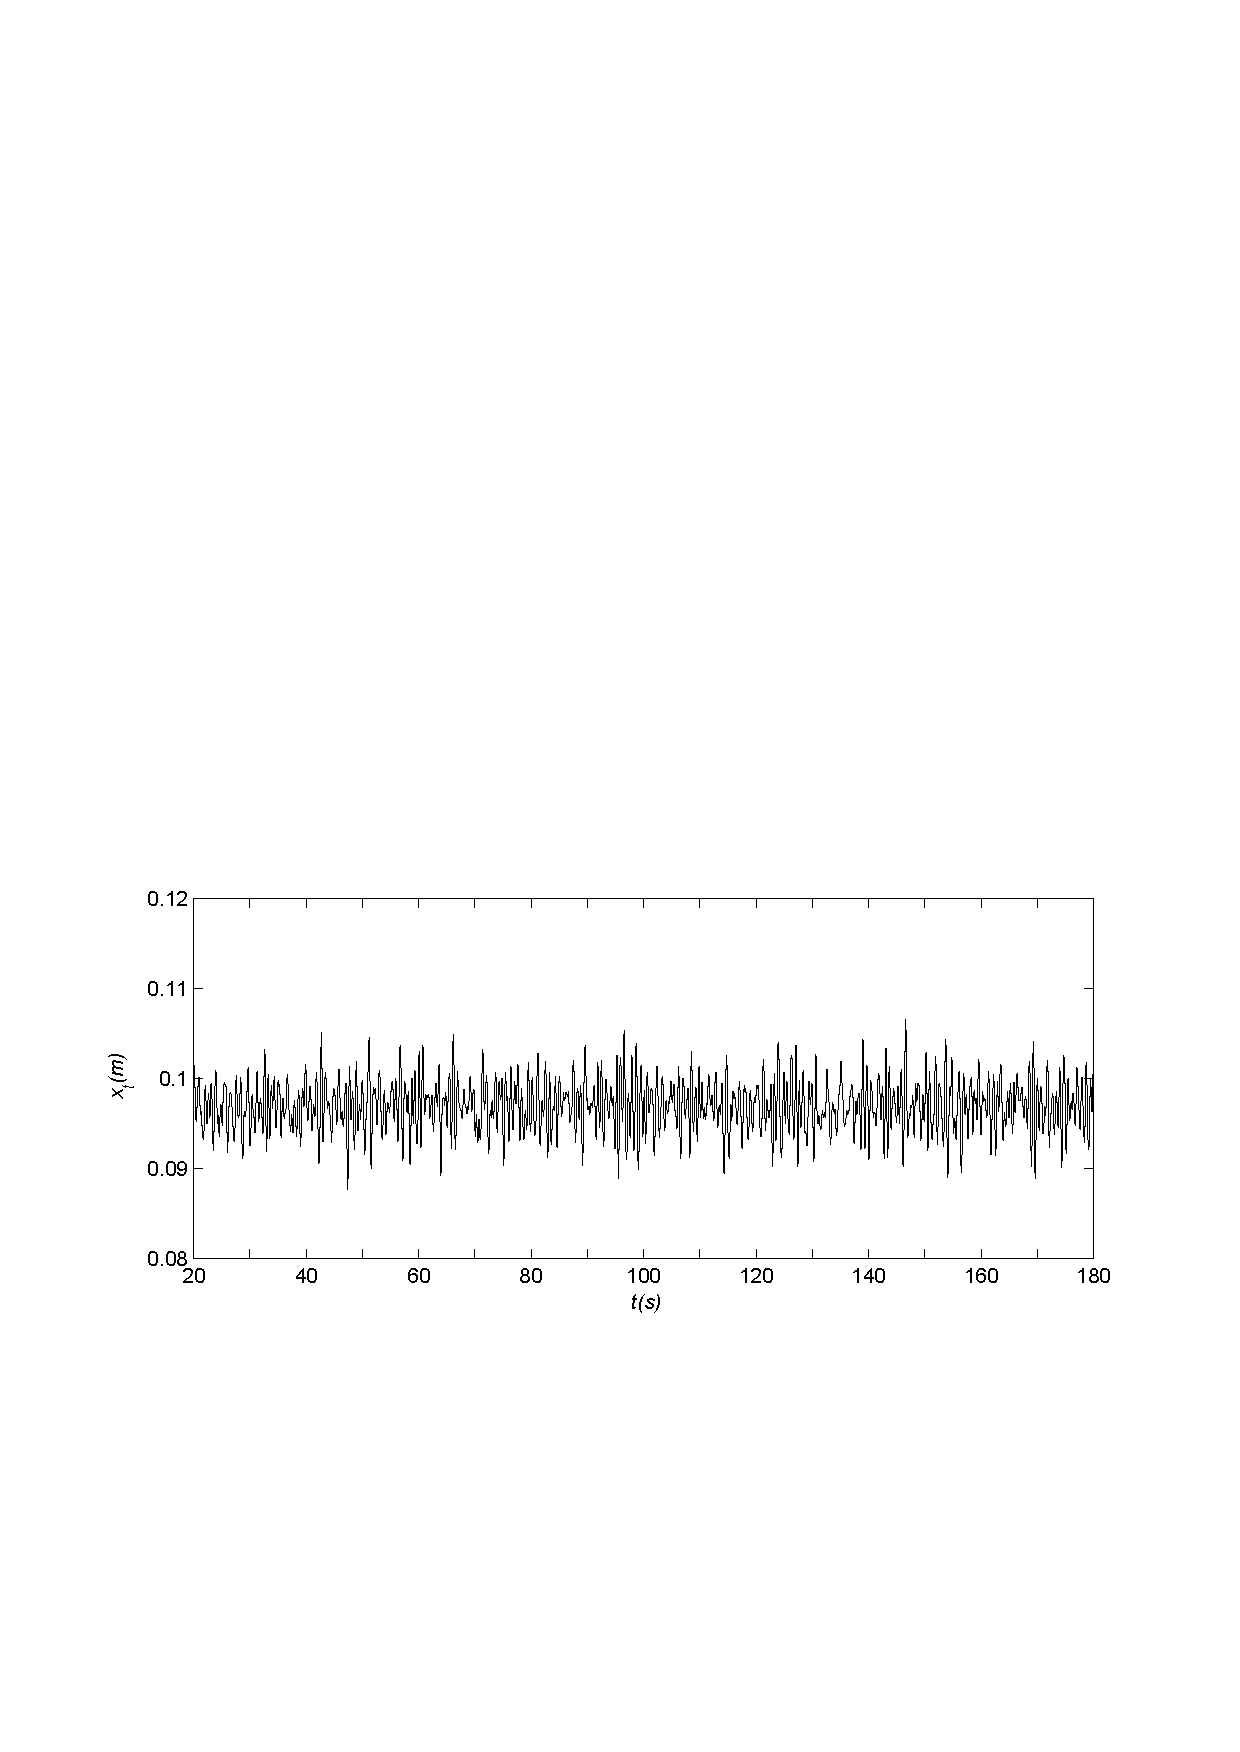
\includegraphics[width=0.8\hsize]{MATLAB-kalman.pdf}
  \caption{Displacement curve of Kalman filter}
  \label{fig:kalman}
\end{figure}

\begin{figure}[H]
  \centering
  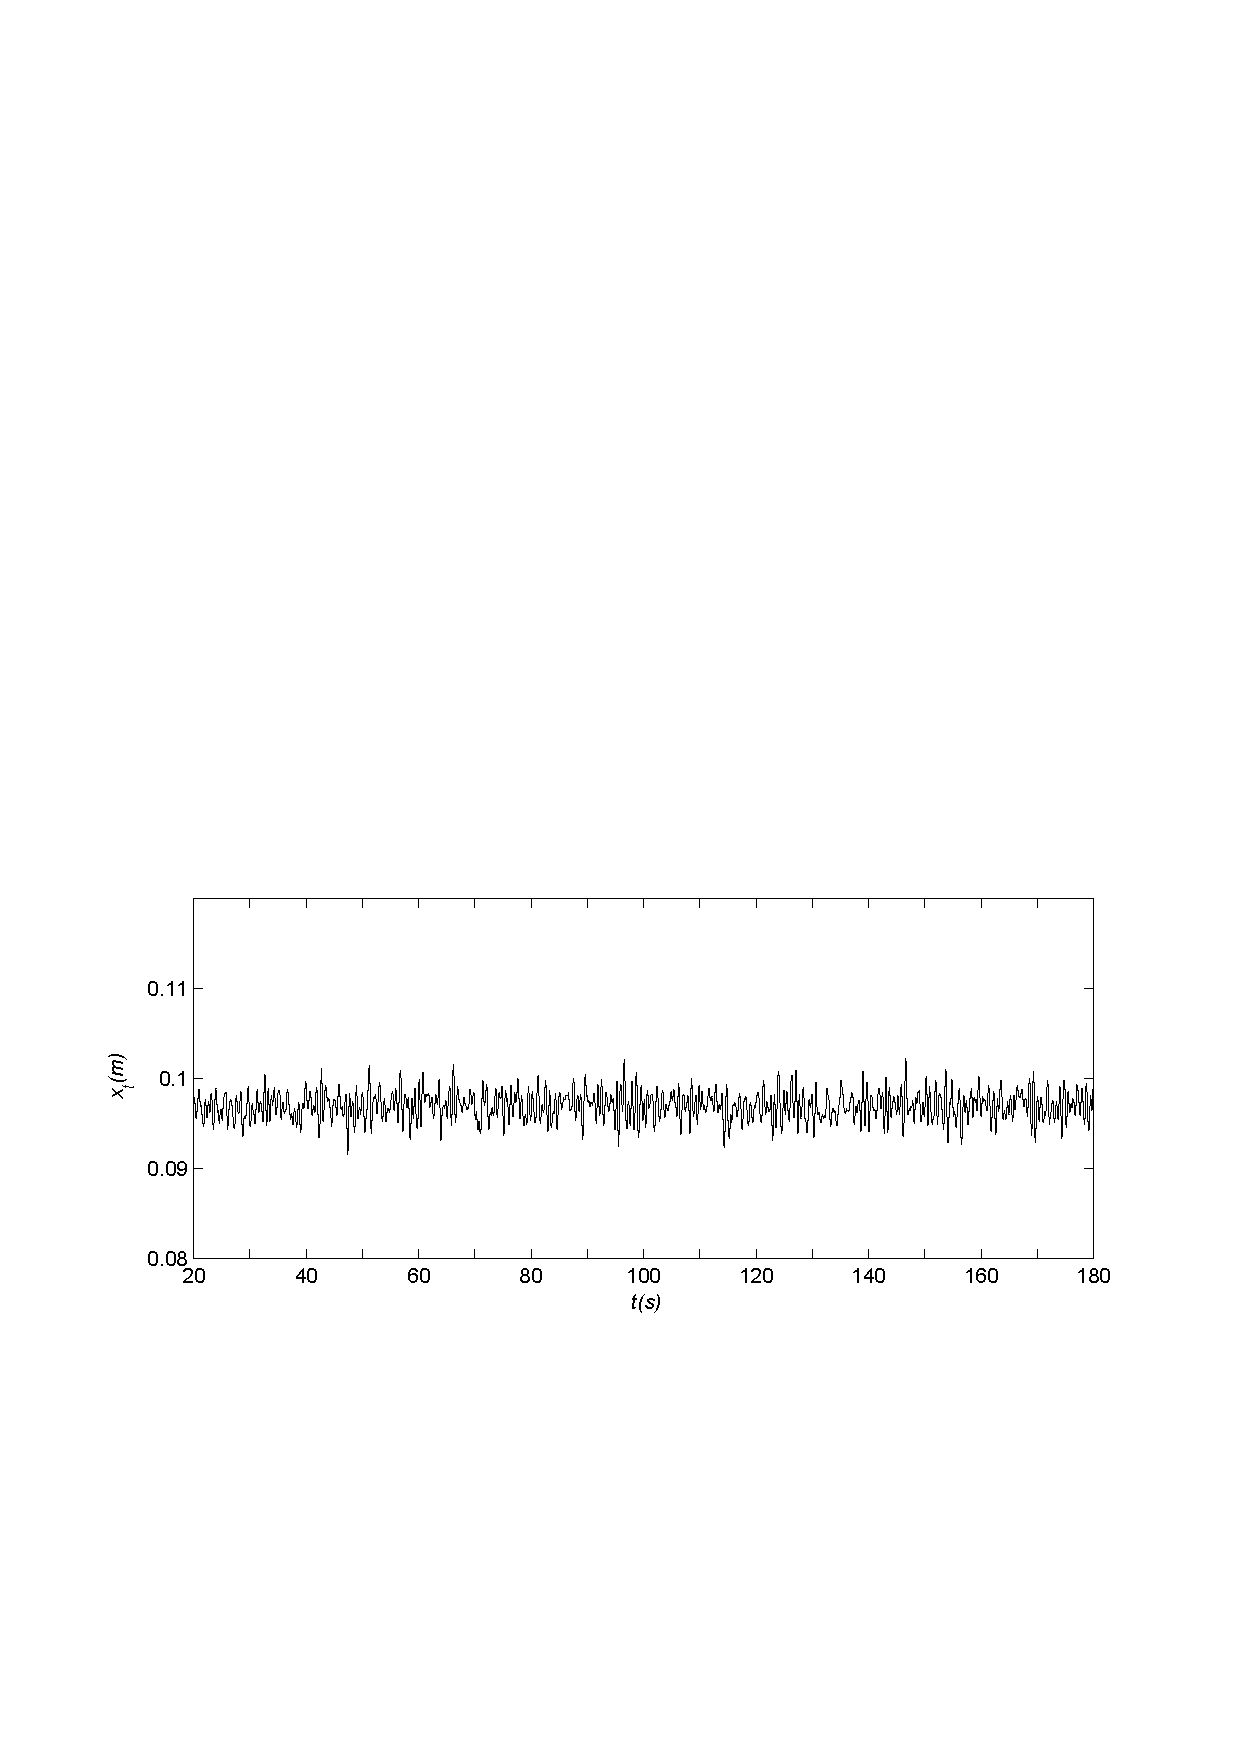
\includegraphics[width=0.8\hsize]{MATLAB-multi.pdf}
  \caption{Displacement curve of the multi-innovation Kalman filter}
  \label{fig:multi}
\end{figure}

\begin{figure}[H]
  \centering
  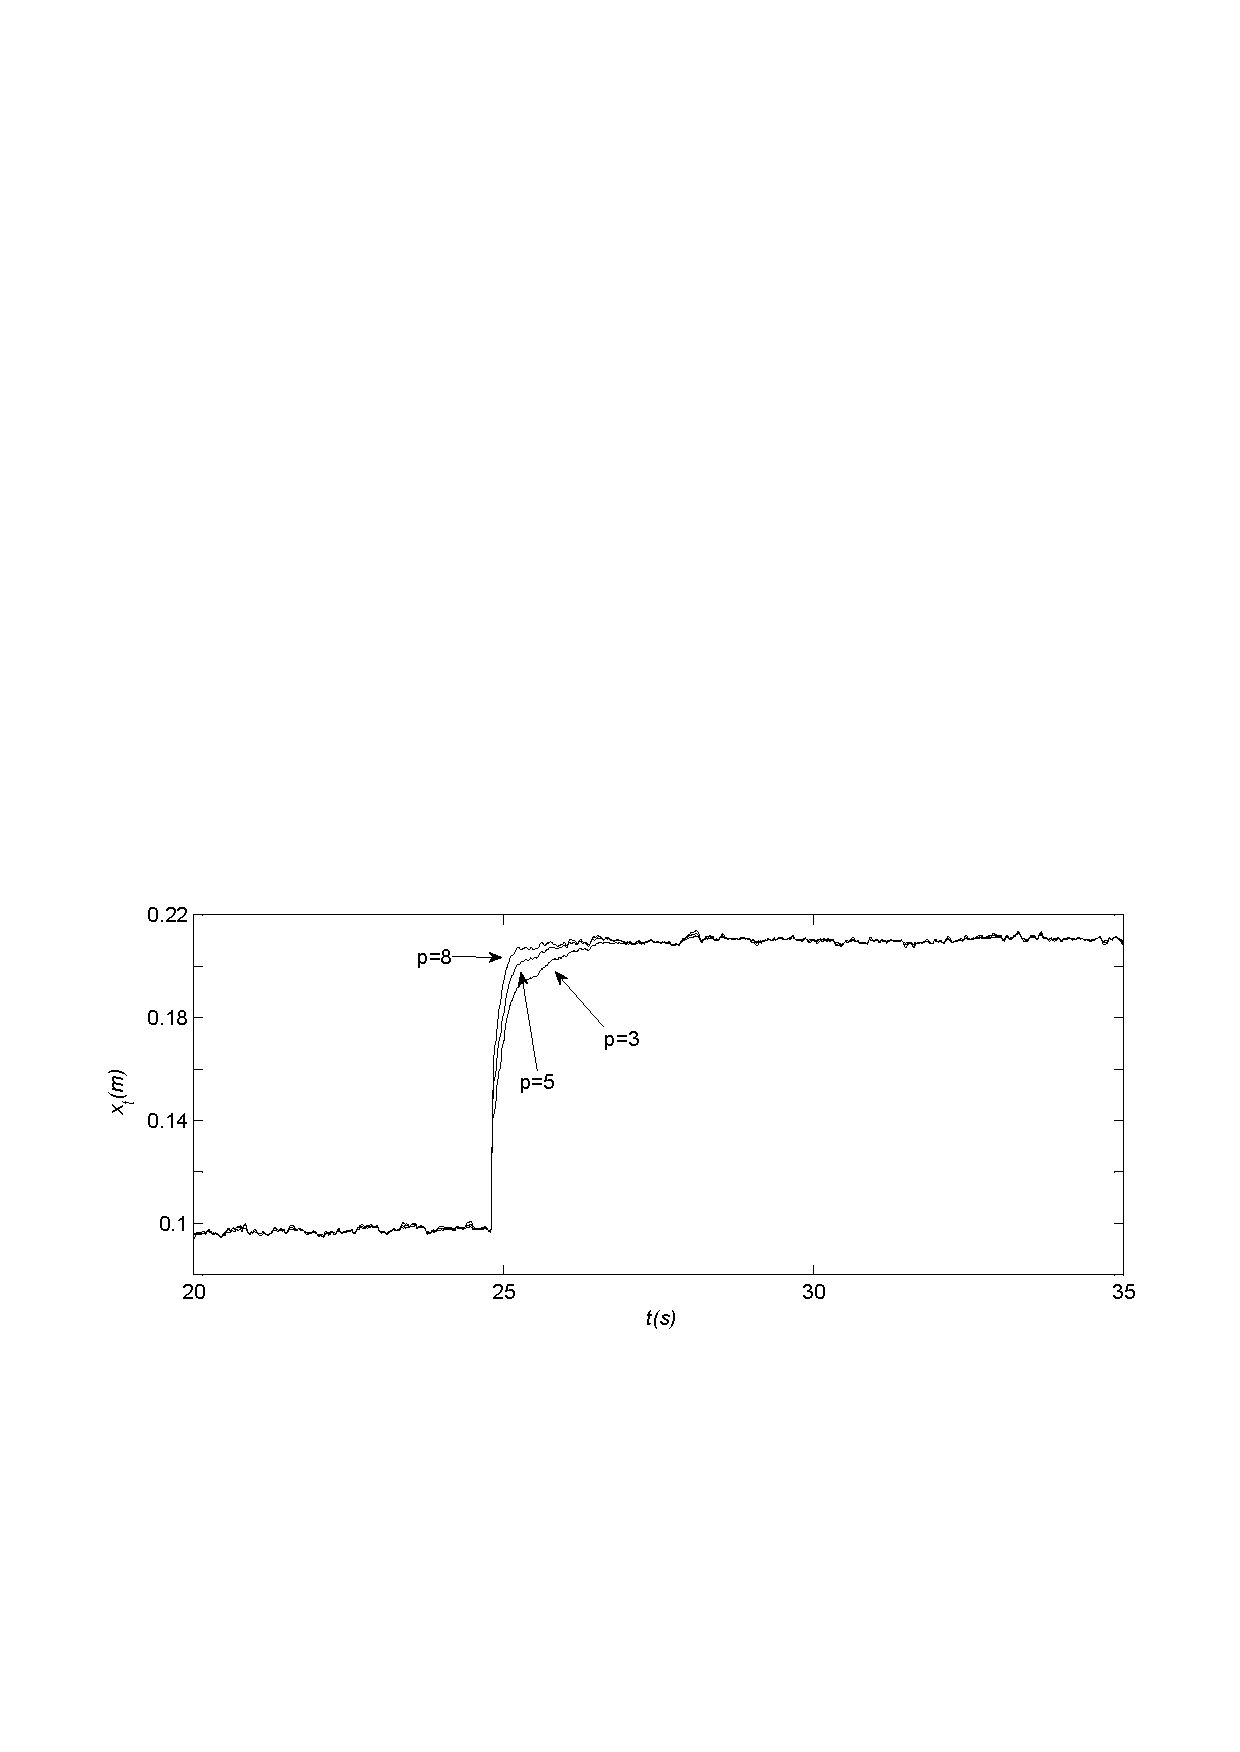
\includegraphics[width=0.8\hsize]{MATLAB-innolength0.pdf}
  \caption{Displacement of the different innovation length}
  \label{fig:innolength0}
\end{figure}

\begin{figure}[H]
  \centering
  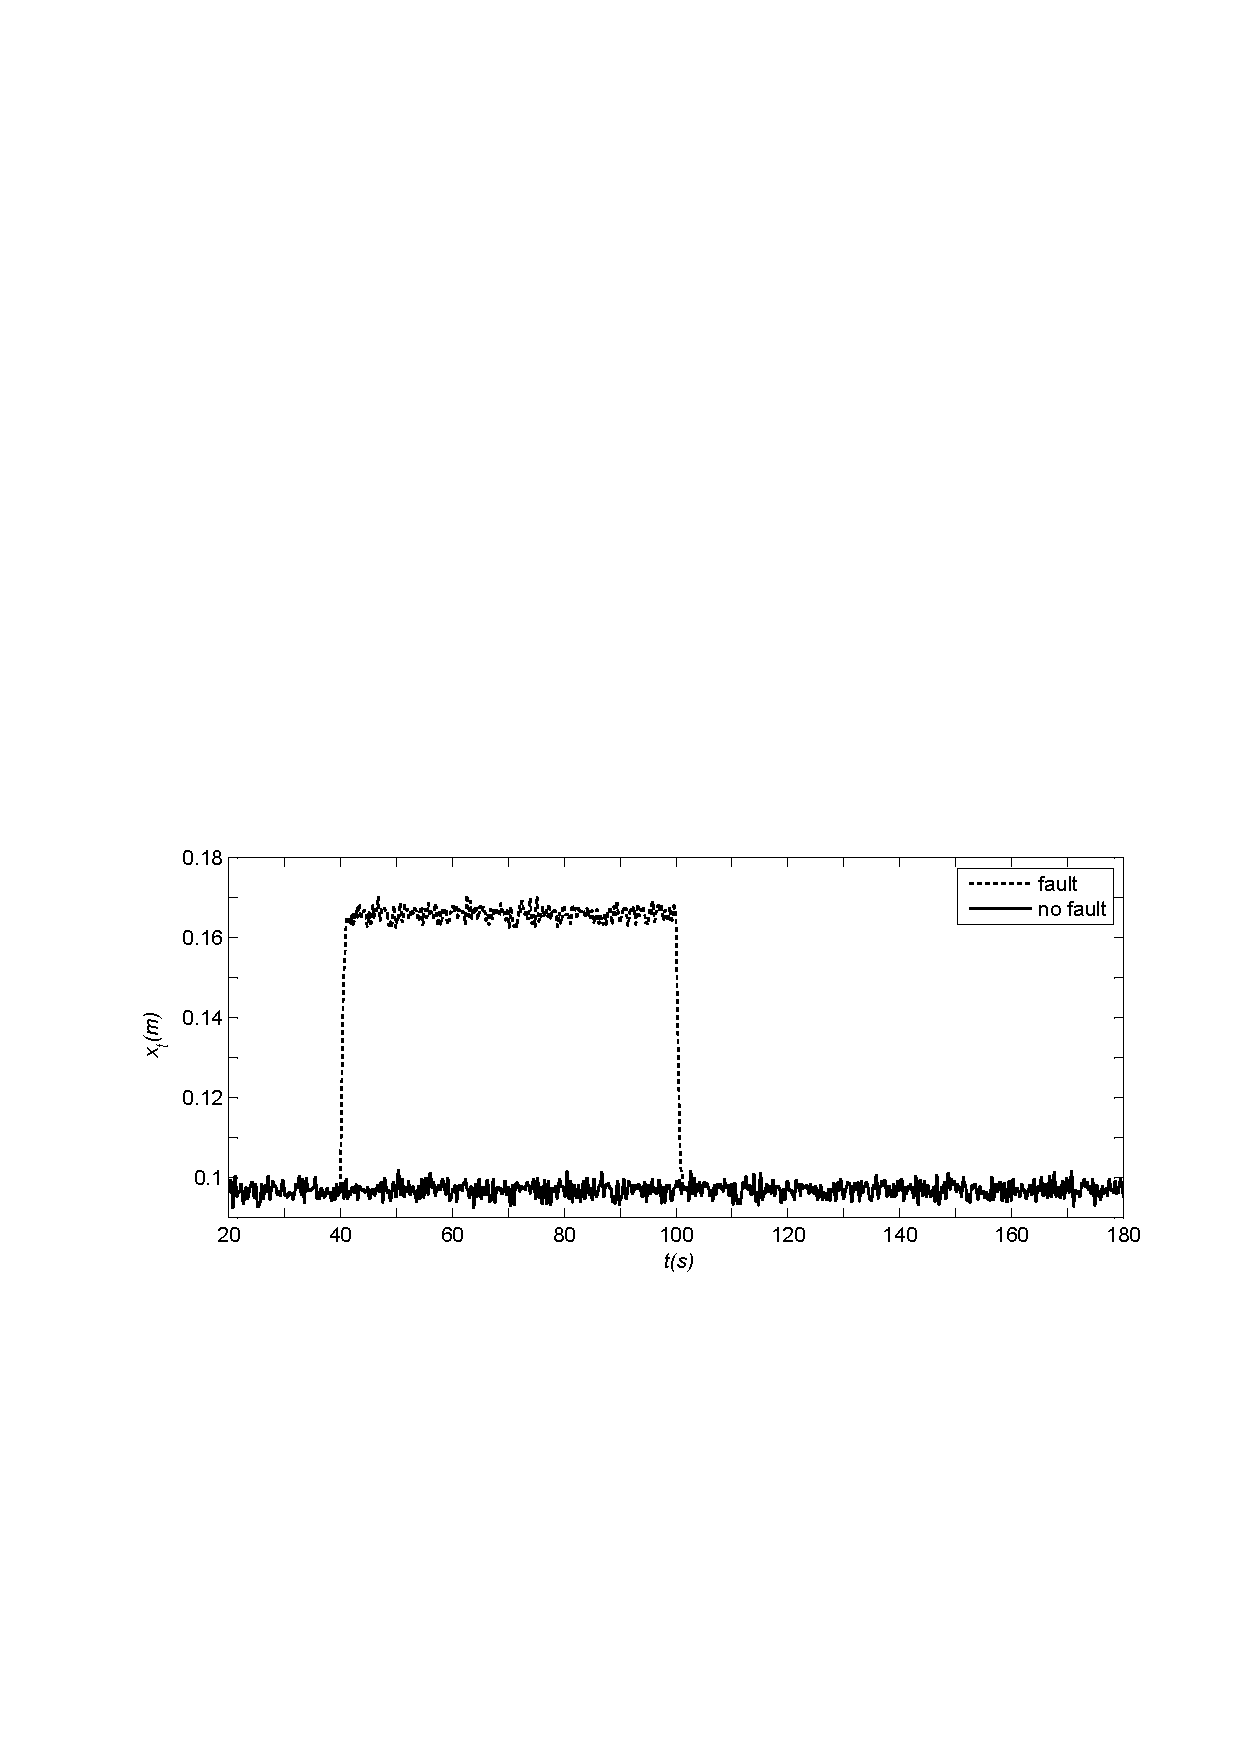
\includegraphics[width=0.8\hsize]{MATLAB-fault1.pdf}
  \caption{Displacement of the fault and fault-free}
  \label{fig:fault1}
\end{figure}

\begin{figure}[H]
  \centering
  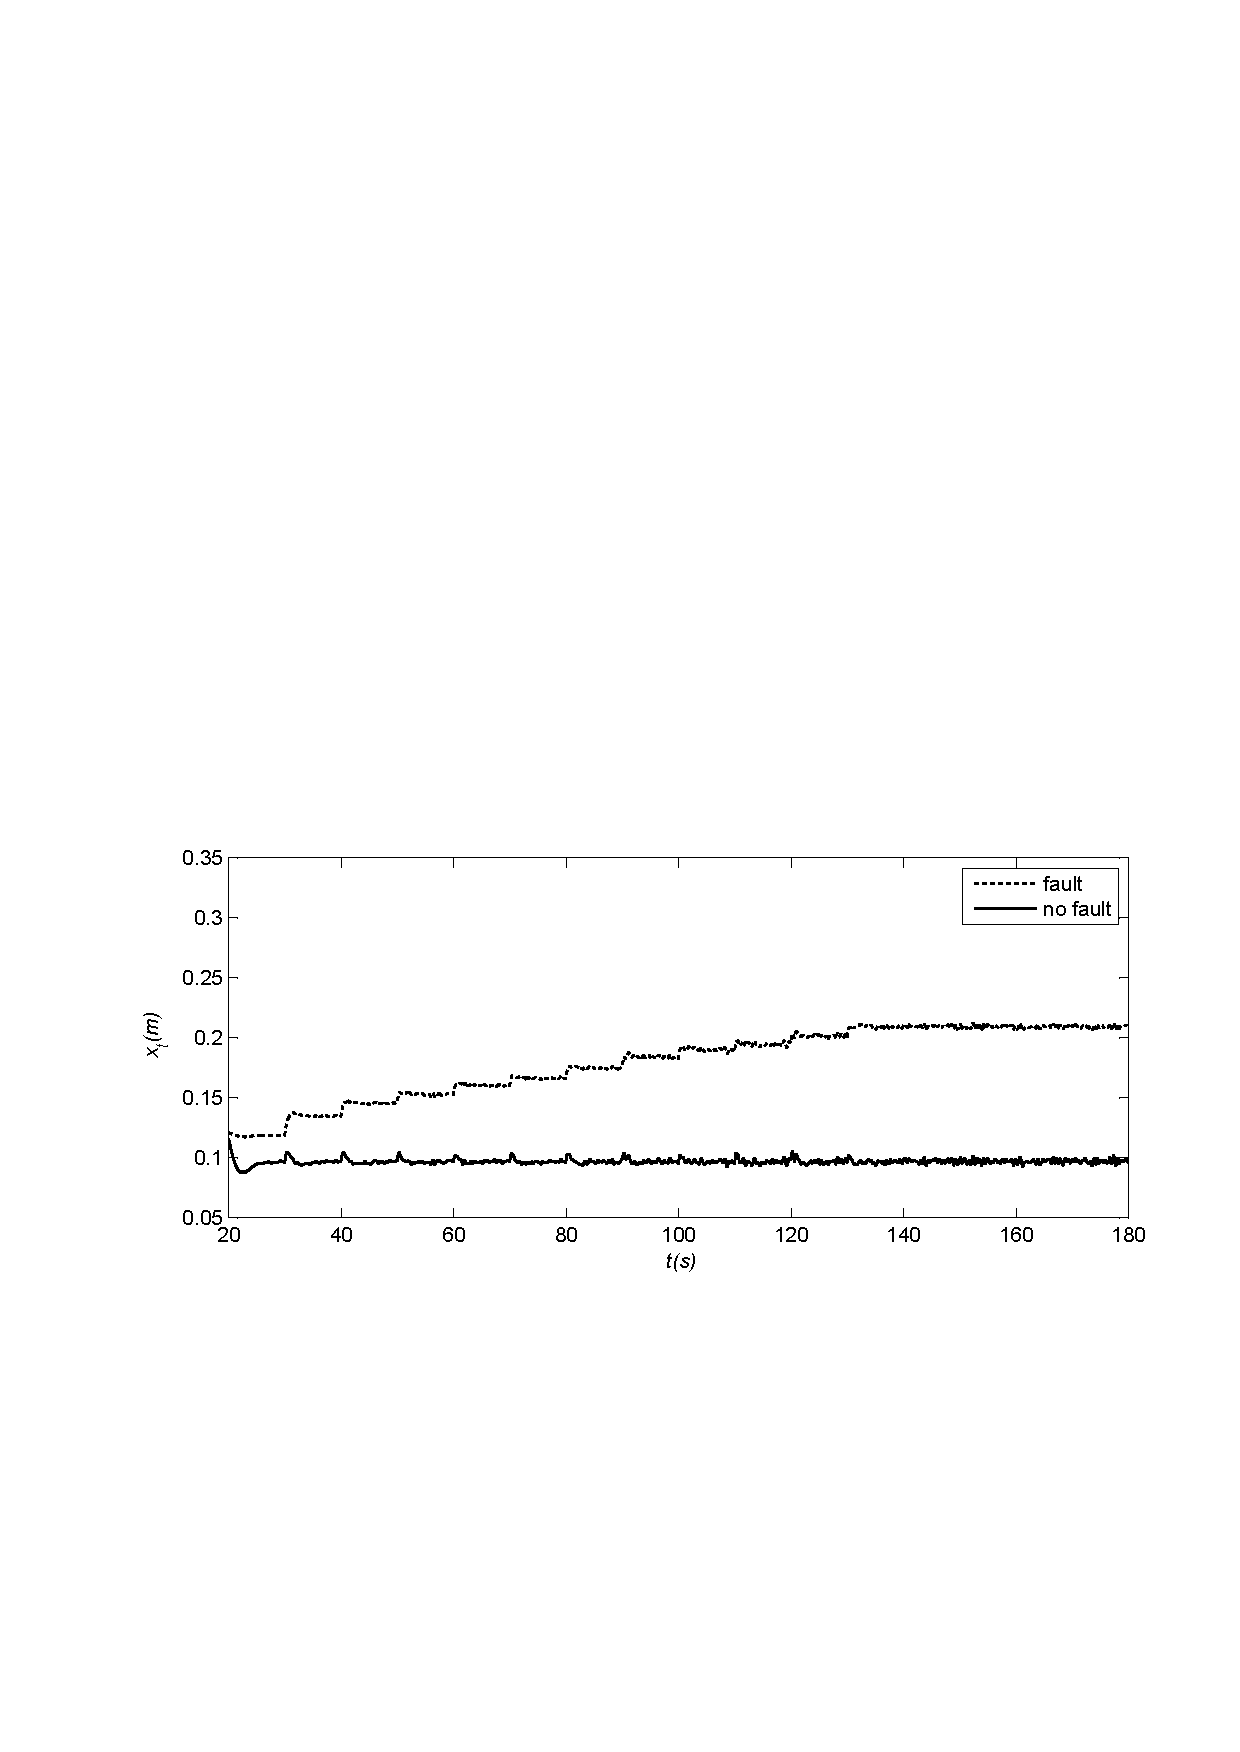
\includegraphics[width=0.8\hsize]{MATLAB-fault5.pdf}
  \caption{Displacement of the different wind velocities}
  \label{fig:fault5}
\end{figure}

\begin{figure}[H]
  \centering
  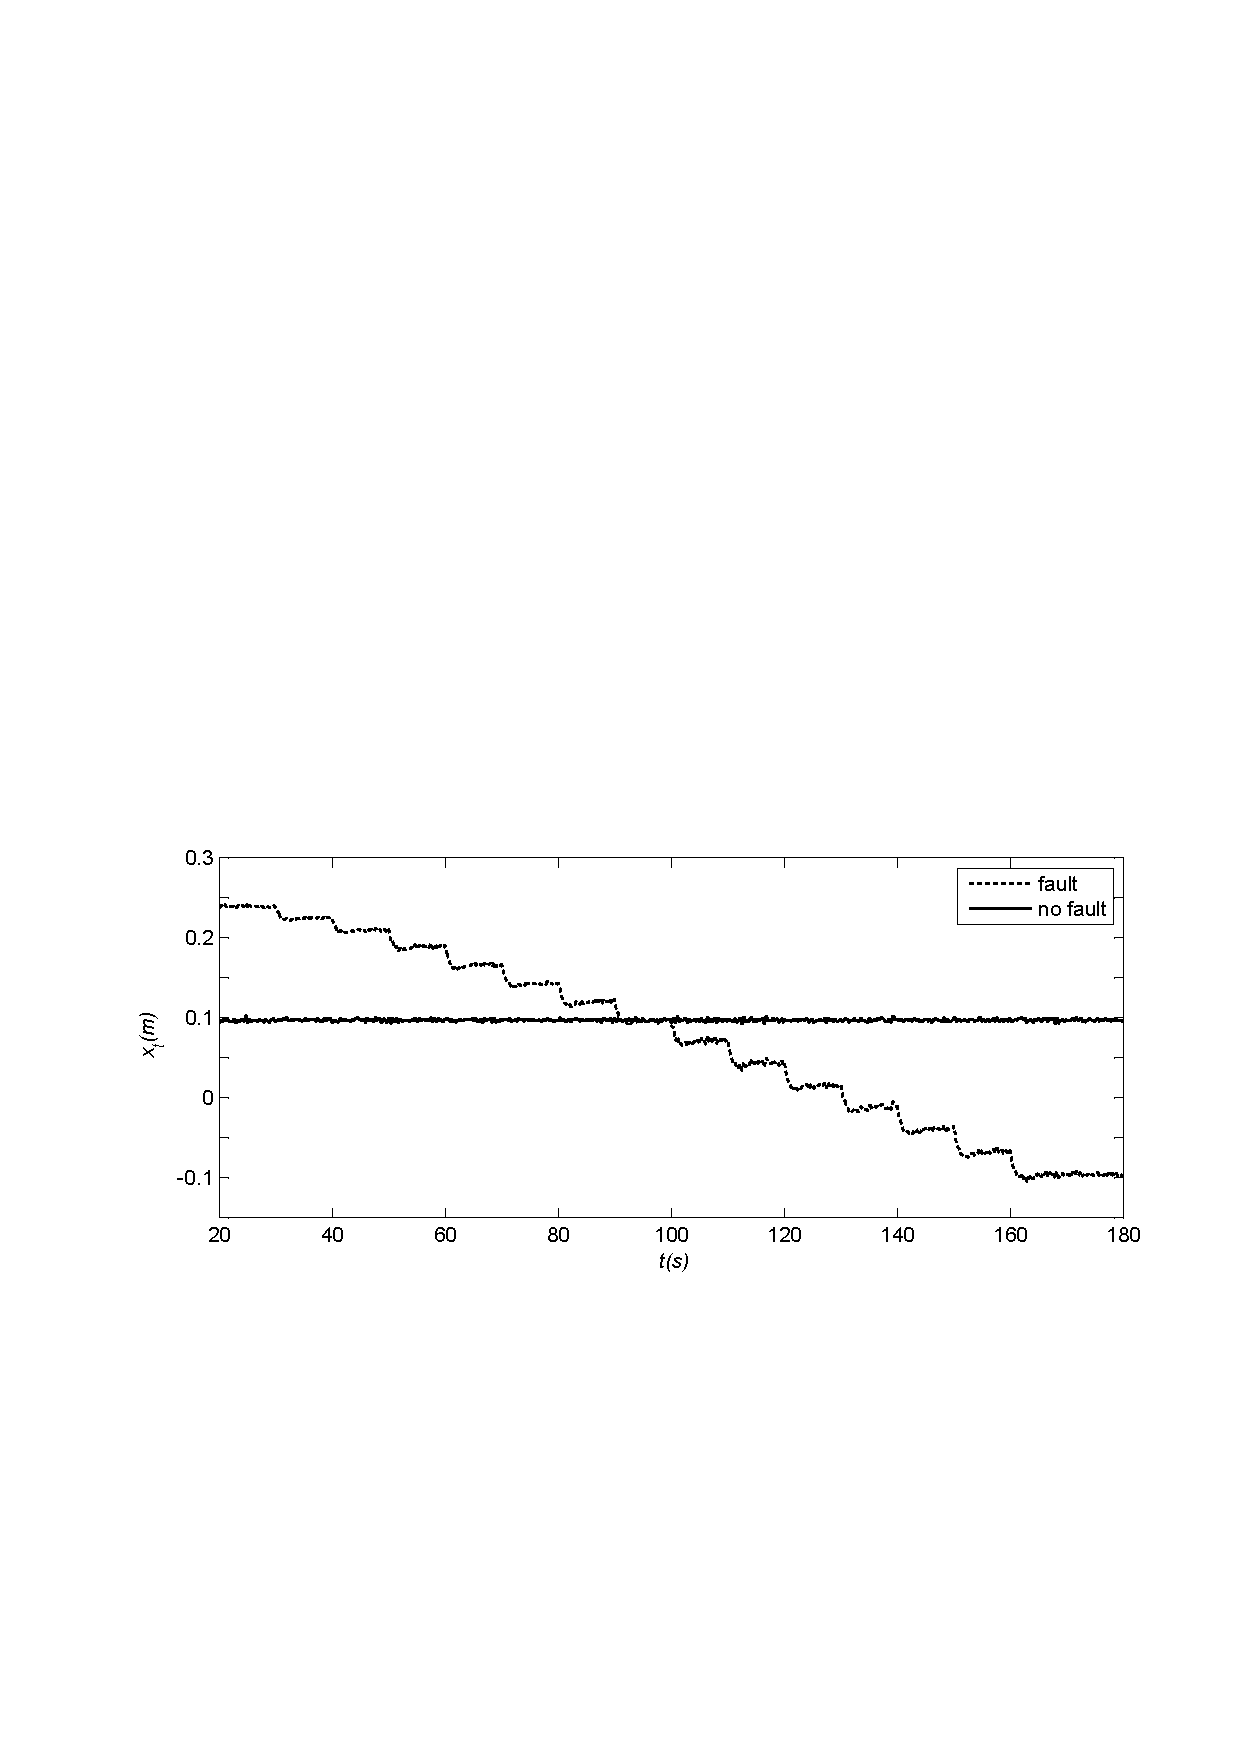
\includegraphics[width=0.8\hsize]{MATLAB-fault25.pdf}
  \caption{Displacement of the different pitch angles}
  \label{fig:fault25}
\end{figure}

\begin{figure}[H]
  \centering
  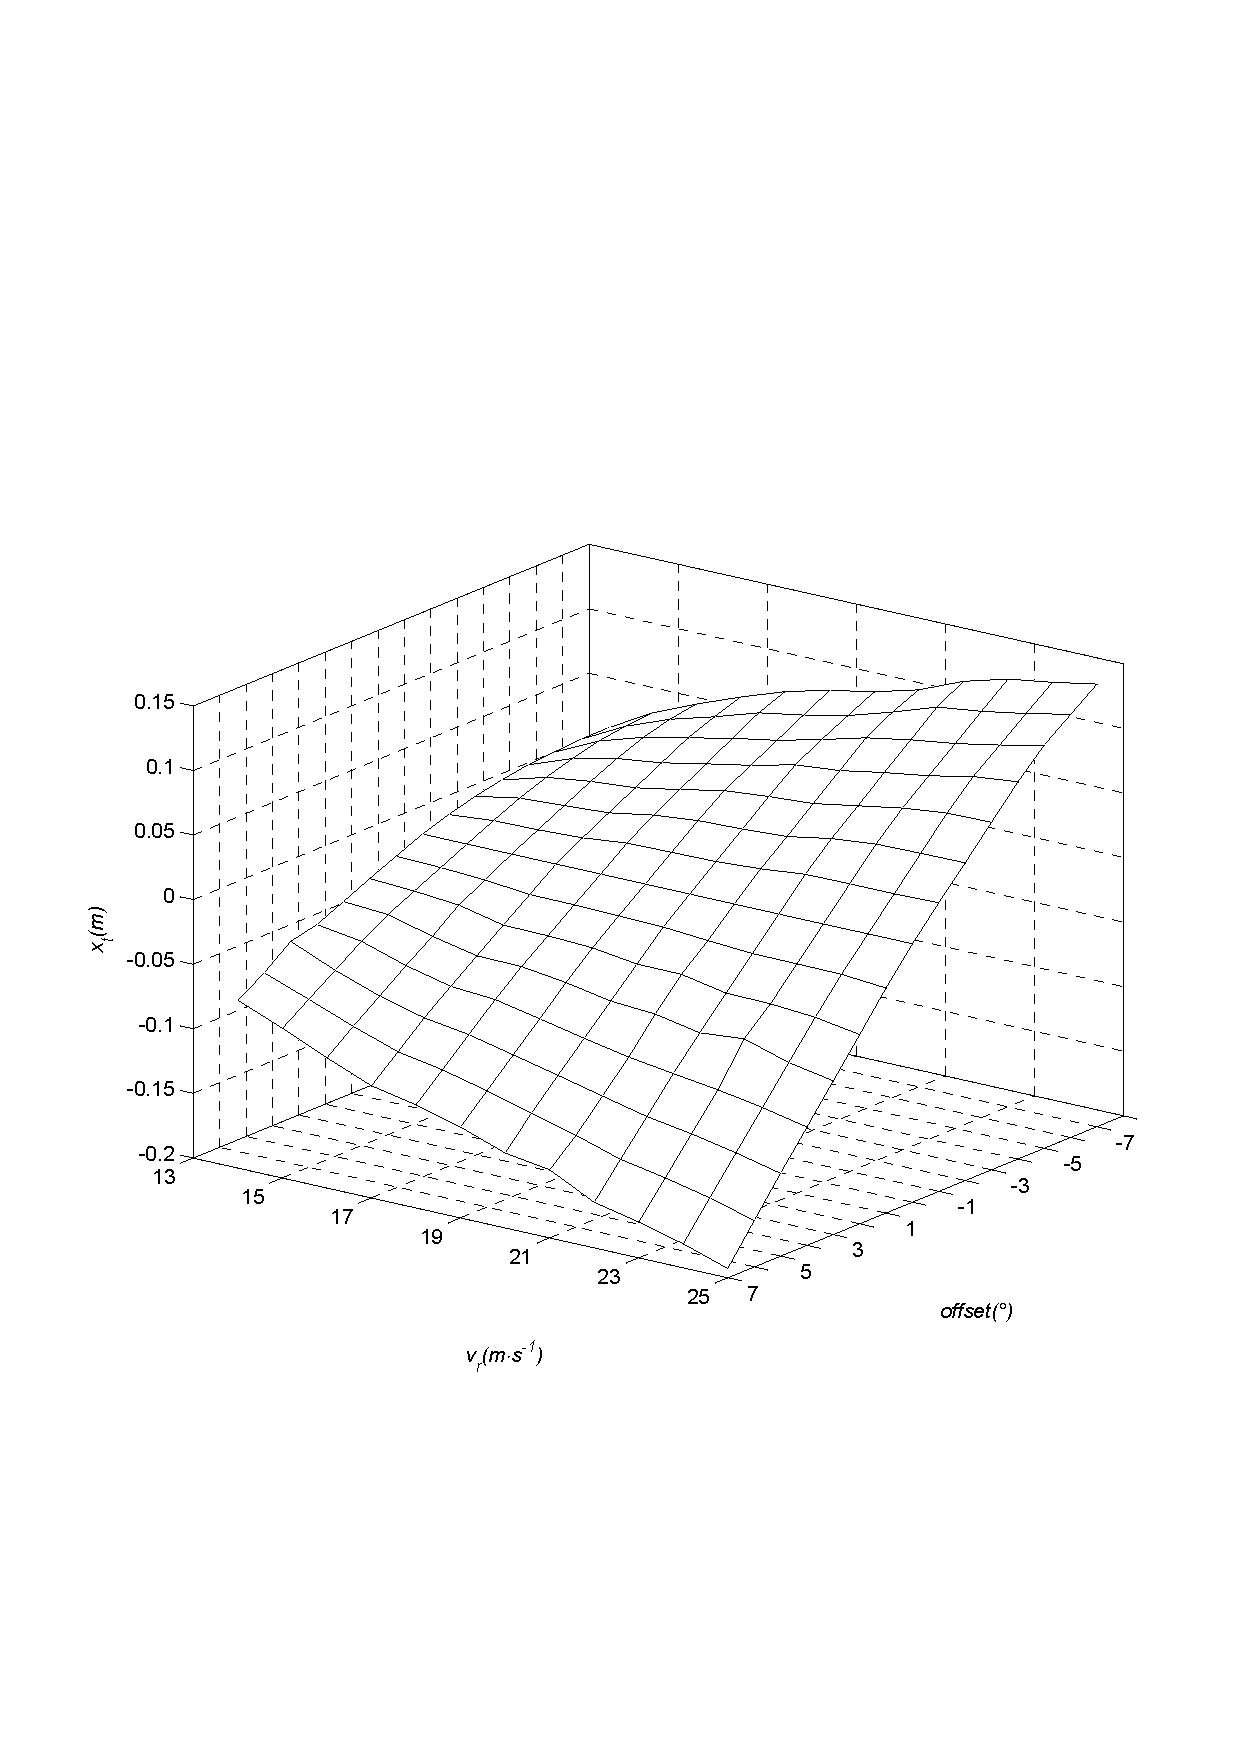
\includegraphics[width=0.9\hsize]{MATLAB-3d.pdf}
  \caption{Wind velocity-pitch angle-displacement}
  \label{fig:3d}
\end{figure}


\section{Conclusion}

In this paper, the pitch angle sensor offset fault is considered,
and a
relationship between the sensor offset and the tiny displacement of
tower is established for fault diagnosis. To obtain more
accurate displacement states, the conventional Kalman filter is
extended to the multi-innovation Kalman filter. The multi-innovation
algorithm shows faster convergence.
It is shown in Fig. \ref{fig:3d} that the sensor offset value
can be estimated from the wind velocity and the displacement
deviation.



%\baselineskip 5pt

%\footnotesize
\clearpage
\begin{thebibliography}{99}
\bibitem{ref:1}
Global Wind Energy Council. Global wind report-annual market update, 2011.

\bibitem{ref:2}
Fu Z X. Status and prospects on condition monitoring technologies of offshaore wind turbine. \emph{Automation of Electric Power Systems}, 2012, 36(1): 121--129.


\bibitem{ref:3}
Li S B, Sauter D, Aubrun C. Stability guaranteed active fault-tolerant control of networked control systems. \emph{Journal of Control Science and Engineering}, 2008; 5: 22--31.

\bibitem{ref:4}
Watson S J, Xiang B J, Yang W, et al. Condition monitoring of the power output of wind turbine generators using wavelets. \emph{IEEE Transactions on Energy Conversion}, 2010, 25(3): 715--721.

\bibitem{ref:5}
Guolian H, Pan J, Zhentao W, et al. Research on fault diagnosis of wind turbine control system based on Artificial Neural Network. \emph{Proceedings of 8th world congress on intelligent control and automation (WCICA2010)}, July 6--9, 2010, Jinan, China, (pp. 4875--4879).

\bibitem{ref:6}
Yao J, Wang J H. Recursive identification of parameters in the minimum variance control. \emph{Proceedings of 10th world congress on intelligent control and automation (WCICA2012)}, July 6--8, 2012, Beijing, China, (pp. 2870--2877).

\bibitem{ref:7}
Munteanu I, Bratcu A I, Cutululis N A, et al. \emph{Optimal control of wind energy systems: towards a global approach}. Springer, 2008.


\bibitem{ref:8}
Esbensen T, Sloth C. Fault Diagnosis and Fault-Tolerant Control of Wind Turbines. \emph{Master's Thesis}, Aalborg University, 2009.

\bibitem{ref:9}
Ding F. Several multi-innovation identification methods. \emph{Digital Signal Processing}, 2010, 20(4): 1027--1039.

\bibitem{ref:10}
Ding F, Liu X P, Liu G. Multi-innovation least squares identification for system modeling. \emph{IEEE Transactions on Systems, Man, and Cybernetics, Part B: Cybernetics}, 2010, 40(3): 767--778.

\bibitem{ref:11}
Han L L, Ding F. Multi-innovation stochastic gradient algorithms for multi-input multi-output systems. \emph{Digital Signal Processing}, 2009, 19(4): 545--554

\bibitem{ref:12}
Ding F, Chen T. Performance analysis of multi-innovation gradient type identification methods. \emph{Automatica}, 2007, 43(1): 1-1-4

\bibitem{ref:13}
Mohammadpour J, Scherer C W. \emph{Control of linear parameter varying systems with applications}. Springer, 2012.

\bibitem{ref:14}
Bianchi F D, De Battista H, Mantz R J. \emph{Wind Turbine Control Systems: Principle, Modeling and Gain Scheduling Design}. Springer, 2007.



\bibitem{ref:15}
Odgaard P F, Johnson K E. Wind turbine fault detection and fault tolerant control-an enhanced benchmark challenge. \emph{Proceedings of American Control Conference (ACC)}, June 17--19, 2013, Washington, America, (pp. 4447--4452).

\bibitem{ref:16}
Kolouri S, Azimi-Sadjadi  M R, Ziemann A. Acoustic Tomography of the Atmosphere Using Unscented Kalman Filter. \emph{IEEE Transactions on Geoscience and Remote Sensing}, 2014, 52(4): 2159--2171.

\bibitem{ref:17}
Ding F. System identification. part F:  multi-innovation identification theory and methods. \emph{Journal of Nanjing University of Information Science and Technolony: Natural Science Edition}, 2012, 4(1): 1--28.





\end{thebibliography}


\end{document}
